\documentclass[11pt,a4paper]{article}
\usepackage[T1]{fontenc}
\usepackage[utf8]{inputenc}
\usepackage{lmodern}
\usepackage[margin=2.6cm]{geometry}
\usepackage{amsmath,amssymb,amsthm}
\usepackage{booktabs}
\usepackage{graphicx}
\usepackage{microtype}
\usepackage[hidelinks,pdfauthor={Oliver D'Souza},
  pdftitle={Guaranteed behaviour of a small trained transformer at every input length: a machine-checked proof of concept}]{hyperref}

\newtheorem{theorem}{Theorem}
\newtheorem{lemma}[theorem]{Lemma}
\newtheorem{proposition}[theorem]{Proposition}
\newtheorem{corollary}[theorem]{Corollary}
\newcommand{\lean}[1]{\texttt{#1}}
\newcommand{\R}{\mathbb{R}}
\newcommand{\cnt}{\#}
\setlength{\emergencystretch}{3em}

\title{Guaranteed behaviour of a small trained transformer\\at every input length:\\a machine-checked proof of concept}
\author{Oliver D'Souza\thanks{Copyright \textcopyright\ 2026 Oliver D'Souza. This paper is licensed under
\href{https://creativecommons.org/licenses/by/4.0/}{Creative Commons Attribution 4.0 International (CC BY 4.0)}.}}
\date{15 November 2026}

\begin{document}
\maketitle

\begin{abstract}
The behaviour of a trained neural network is usually estimated by testing; this
paper is a proof of concept for guaranteeing it by a machine-checked proof about
the trained weights. The network is a one-layer, one-head, attention-only
transformer without positional embeddings, trained at length 10 to output the
largest of its input tokens. We prove in Lean~4, using only Lean's standard
axioms, statements about what it computes on inputs of every length. The
certified model has weights rounded to multiples of $2^{-10}$ and exact
real-valued softmax; the proofs work from its attention and value tables and
never enumerate inputs.
First, the model is correct whenever the other tokens are few enough and far
enough below the maximum: for example, on any number of copies of a maximum of
at least 23 together with at most $10^6$ other tokens, each at least 16 below
it. Second, it is provably wrong on explicit inputs, among them inputs of the
training length, although it answers all of $2^{19}$ random inputs of that
length correctly. Third, the two kinds of statement meet in exact thresholds:
on $k$ copies of 20 followed by 21 the model answers 21 if and only if
$k\le4$, and in each of five training seeds, at every gap $g\le6$ and for at
least 39 of the 40 maxima $m$ from 24 to 63, there is an explicit $N$ such that
the model is correct with up to $N$ other tokens at most $m-g$ and wrong on
every larger number of copies of $m-g$. All theorems are checked by the Lean
kernel from the weight matrices up, in under an hour per model on a desktop
computer. Code, weights and proofs:
\url{https://github.com/Oliverds321/transformer-all-lengths-lean}.
\end{abstract}

\section{Introduction}

What a trained neural network does on inputs it was not tested on is, as a
rule, not known but estimated. Proposals for AI systems with guaranteed
behaviour~\cite{tegmark2023provably,dalrymple2024gsai} ask for more: a formal
statement of the intended behaviour and a proof, checkable by a small trusted
program, that the system satisfies it. For neural networks themselves such
proofs are rare. Verification tools establish properties of fixed-size networks
over bounded input regions, transformers
included~\cite{shi2020robustness,bonaert2021deept}. Statements about what a
trained transformer computes over its whole input space, let alone over inputs
of unbounded length, have, with few exceptions, not been machine-checked
(Section~\ref{sec:related}).

The starting point of this paper is mechanistic interpretability, which
explains a trained network by describing an algorithm that its weights
implement. Such an explanation is usually tested on samples. Gross et
al.~\cite{gross2024compact} proposed a stricter test: use the explanation to
\emph{prove} a bound on the accuracy of the network, at a cost well below that
of running it on every input. They did this for small transformers trained on
Max-of-$K$ (output the largest of $K$ tokens), with computer-assisted proofs in
Python whose arithmetic is floating point.

We take the same task and make two changes. The first is the standard of proof:
every statement is a theorem of Lean~4, checked by its kernel (the small trusted
core of Lean that checks every proof) with only the standard axioms
\lean{propext}, \lean{Classical.choice} and \lean{Quot.sound}, about a
transformer that is defined inside Lean from its weight matrices with
real-valued softmax. The second is the kind of statement. Without positional
embeddings, one set of weights defines a function on input sequences of every
length~\cite{kazemnejad2023nope}, and we prove statements quantified over all
lengths: a region in which the model is correct, explicit inputs on which it is
wrong, and exact thresholds between the two.

This is a proof of concept that such statements are within reach. The model and
the task are chosen to be as simple as possible, so that the whole chain, from
the weight matrices to the final theorems, can be checked and inspected.
Section~\ref{sec:limits} discusses what larger models would need.

\paragraph{What is proved.}
For a model trained at length 10 (vocabulary 64, embedding dimension 32):
\begin{itemize}
\item \emph{Correctness at every length} (Theorem~\ref{thm:gap}). Six statements
of the form: if the maximum is at least $m_0$, every other token is at least $g$
below it, and at most $N$ positions before the last hold a token other than the
maximum, then the logit of the maximum is strictly larger than every other
logit. The number of copies of the maximum is not bounded, so each statement
covers inputs of every length. The triples $(N,g,m_0)$ range from $(3,1,15)$ to
$(10^6,16,23)$.
\item \emph{Failures from an explicit length on} (Theorem~\ref{thm:fail}). For
53 values of the maximum $m$, among them every $m\ge15$, an explicit
$k_0(m)\le17$ such that for every $k\ge k_0(m)$ the model does not answer $m$
on $k$ copies of $m-1$ followed by $m$.
\item \emph{Exact thresholds} (Theorem~\ref{thm:tight}). For 613 of the 640
pairs of a maximum $m$ from 24 to 63 and a gap $g$ from 1 to 16, an explicit
$N(m,g)$ such that the model answers $m$ whenever its last token is $m$ and at
most $N(m,g)$ positions hold other tokens, all at most $m-g$, and does not
answer $m$ on more than $N(m,g)$ copies of $m-g$ followed by $m$.
\item \emph{Accuracy at fixed lengths} (Theorem~\ref{thm:acc}): lower bounds
$0.9972$, $0.9705$, $0.8841$ and $0.5203$ on the fraction of all inputs of
length 4, 10, 20 and 100 that are answered correctly.
\item \emph{A fixed-length baseline} (Theorem~\ref{thm:k4}): for a model with
positional embeddings trained at length 4, at least $16{,}777{,}215$ of the
$64^4=16{,}777{,}216$ inputs are answered correctly.
\end{itemize}
Analogous statements, with their own constants, are proved for four further
training seeds.

The thresholds show that the correctness statements cannot be improved for
these inputs. On $k$ copies of 20 followed by 21, for example, the model
answers 21 if and only if $k\le4$. In every seed, at every gap up to 6, such an
exact threshold is proved for at least 39 of the 40 maxima
(Figure~\ref{fig:gap}).

The failures are not artefacts of extreme lengths: for the maximum 21 they begin
at length 6, and for every maximum from 15 to 63 by length 18, so they include
inputs of the training length. Yet on $2^{19}$ uniformly random inputs of
length 10, the model of every seed answered every input correctly: inputs of
the form $(m-1)^k\,m$ are a vanishing fraction of random ones. A proof about
the weights finds them.

\paragraph{Contribution and scope.}
The contribution is the instance: machine-checked statements about the weights
of a trained attention model that hold at every input length, in both
directions and with exact thresholds, proved in exact arithmetic. The model is
deliberately minimal, and the proof builds on known ingredients. The key
identity (Lemma~\ref{lem:sep}) is implicit in the convexity argument
of~\cite{gross2024compact}; that such a model sees only token counts follows
from the path expansion of~\cite{elhage2021mathematical} (see
also~\cite{salzer2026counting}); and the dispersion of softmax attention with
length, which underlies both the correctness region and the failures, was
proved in general by Veli\v{c}kovi\'c et al.~\cite{velickovic2025softmax}. The
theorems are about the quantised model defined in Section~\ref{sec:model}.

\section{The model}\label{sec:model}

Tokens are the numbers $0,\dots,V-1$ with $V=64$. An input is a sequence
$s=(t_1,\dots,t_n)$ of length $n$; the last token $q=t_n$ is called the
\emph{query}. The model has a token embedding $E\in\R^{V\times d}$ ($d=32$),
optionally a positional embedding $P\in\R^{n\times d}$, matrices
$W_Q,W_K,W_V,W_O\in\R^{d\times d}$ and an unembedding $W_U\in\R^{d\times V}$.
With $x_i=E_{t_i}+P_i$ it computes
\[
 \sigma_i=(x_nW_Q)\cdot(x_iW_K),\qquad
 \alpha=\operatorname{softmax}(\sigma),\qquad
 \ell=\Bigl(x_n+\sum_{i=1}^n \alpha_i\,x_iW_VW_O\Bigr)W_U\in\R^V .
\]
There are no biases, no layer normalisation and no MLP. The model is trained
with cross-entropy to make $\ell$ largest at $\max_i t_i$, on uniformly random
sequences of a fixed length; during training the scores are divided by
$\sqrt d$. We say that the model \emph{answers} $m$ on $s$ if $\ell_j<\ell_m$
for every $j\ne m$; a tie counts as a wrong answer. All theorems are about this
relation with $m=\max_i t_i$.

With learned absolute positional embeddings the model is not even defined beyond
its training length. Without them ($P=0$) the same weights apply at every
length, and models of this kind are a studied choice for length
generalisation~\cite{kazemnejad2023nope}. The price is that the model sees only
the token counts and which token is last (Corollary~\ref{cor:counts}).

\paragraph{Quantisation.}
After training, the factor $1/\sqrt d$ is folded into $W_Q$ and every weight is
rounded to the nearest multiple of $1/S$, $S=2^{10}$. The \emph{quantised
model} is the model above with these rational weights and exact real
arithmetic, including the exponentials in the softmax. It is defined in Lean
(\lean{Transformer}, \lean{IntWeights.toTransformer}) from integer matrices
stored as literals, and every theorem is about it. As a check outside the
proofs, we evaluated the quantised model and the floating-point checkpoint,
both in double precision. On $2^{19}$ uniformly random inputs of length 10, and
again of length 100, their predicted tokens agreed on every input, for each of
the five seeds of Section~\ref{sec:results}. On all $64^4$ inputs of length 4
they differed on between 36 and 462 inputs, depending on the seed.

\section{Two facts and the mechanism}\label{sec:facts}

The logits depend on the weights through three tables: the score
$\sigma(q;t,i)$ of the query token $q$ on token $t$ at position $i$, the value
$\nu(t,i;j)$ that token $t$ at position $i$ contributes to logit $j$ through the
head, and the direct term $\delta(q;j)$:
\[
 \ell_j=\delta(q;j)+\frac{\sum_i e^{\sigma(q;t_i,i)}\,\nu(t_i,i;j)}{\sum_i e^{\sigma(q;t_i,i)}} .
\]
Each table is a product of weight matrices (\lean{Transformer.logit\_eq}).

\begin{lemma}[Separability; \lean{Tables.logit\_lt\_iff}]\label{lem:sep}
For tokens $m\ne j$ put
\[\gamma_{q,m,j}(t,i)=\nu(t,i;m)-\nu(t,i;j)+\delta(q;m)-\delta(q;j).\]
Then
\[
 \ell_j<\ell_m\quad\Longleftrightarrow\quad \sum_{i=1}^n e^{\sigma(q;t_i,i)}\,\gamma_{q,m,j}(t_i,i)>0 .
\]
\end{lemma}
\begin{proof}
$\ell_m-\ell_j$ equals the sum on the right divided by $\sum_ie^{\sigma_i}>0$,
because the attention weights sum to one.
\end{proof}

The right-hand side is a sum over positions of a function of the token at that
position (and of $q$, $m$, $j$). Hence the sequence that minimises it within a
set described position by position can be found one position at a time. This is
the convexity argument of~\cite{gross2024compact}; unlike bounds that treat
attention and values separately, it loses nothing.

\begin{corollary}[Counts; \lean{IntPF.answers\_iff\_counts}, \lean{PF10.netAnswers\_iff\_counts}]\label{cor:counts}
Without positional embeddings the tables do not depend on the position $i$,
which we drop. Let $\cnt_t(s)$ be the number of positions of $s$ holding the
token $t$ (the query included). The model answers $m$ on $s$ if and only if for
every $j\ne m$
\[
 \sum_{t} \cnt_t(s)\; e^{\sigma(q;t)}\,\gamma_{q,m,j}(t)>0 .
\]
\end{corollary}

So on every input of every length, correctness is decided by $V-1$ homogeneous
linear inequalities in the token counts, with coefficients that depend on the
query and the maximum: the model is a function of the bag of tokens and of the
last token. Linear inequalities in token counts are central to the study of
what transformers can express~\cite{salzer2026counting}. Since the inequalities
are homogeneous, an input on which the model is wrong remains one when every
count is multiplied by the same integer.

\paragraph{The mechanism.}
The corollary reads as a weighted vote. Each position votes for the right answer
$m$ against a wrong answer $j$ with weight $e^{\sigma(q;t)}$ and sign and size
$\gamma_{q,m,j}(t)$. In the trained model (seed 0), the attention score of a
query $q\ge15$ is largest on the token $q$ itself among the tokens up to $q$,
and for $q\ge20$ it rises over the ten tokens below $q$ by $1.15$ to $2.0$ per
unit of token value on average; and the value of every token from 15 upwards raises that
token's own logit more than any other. So a copy of the maximum casts a heavy
vote for itself, and a token $g$ below it casts a vote whose weight is smaller
by a factor that grows exponentially in $g$. The model is right when the votes
of the maximum outweigh the rest. Because softmax normalises over all
positions, enough copies of a slightly smaller token outvote it, and the model
fails. The region certificates below bound the worst case of this vote; the
failure certificates exhibit a losing one.

\section{Certificates}\label{sec:cert}

A \emph{certificate} is a finite list of integer inequalities. An untrusted
Python program, the \emph{generator}, computes them from the weights; Lean
checks them by evaluation, and a proved soundness lemma turns them into a
theorem. The only analytic ingredient is a rigorous integer interval around
each exponential $e^{\sigma}$. Details that are not needed to follow the results
are in Appendix~\ref{app:cert}.

All tables of the quantised model are integers over the common denominator
$D=S^4$: $\sigma=A/D$, $\nu=B/D$, $\delta=U/D$ (scores and values are products
of four weight matrices; the direct term is a product of two, and $U$ carries
the extra factor $S^2$). Put
$v_j(t)=D\,\gamma_{q,m,j}(t)\in\mathbb Z$. For each query $q$ the kernel checks
natural numbers $\mathrm{lo}_{q,t}\le 2^{F}\exp((A_{q,t}-\bar A_q)/D)\le
\mathrm{hi}_{q,t}$, with $F=256$ and a reference score $\bar A_q\ge A_{q,t}$
(Appendix~\ref{app:cert}). For a token $t$ define the integers
\[
 w^-_j(t)=\begin{cases}\mathrm{lo}_{q,t}\,v_j(t)&v_j(t)\ge0\\ \mathrm{hi}_{q,t}\,v_j(t)&v_j(t)<0\end{cases}
 \qquad
 w^+_j(t)=\begin{cases}\mathrm{hi}_{q,t}\,v_j(t)&v_j(t)\ge0\\ \mathrm{lo}_{q,t}\,v_j(t)&v_j(t)<0.\end{cases}
\]
Then (\lean{IntPF.wLo\_le}, \lean{IntPF.le\_wHi})
\[
 w^-_j(t)\;\le\; \kappa_q\,e^{\sigma(q;t)}\gamma_{q,m,j}(t)\;\le\; w^+_j(t),
 \qquad \kappa_q=2^Fe^{-\bar A_q/D}D>0 ,
\]
so $w^\pm_j(t)$ bound the vote of one copy of $t$, up to a common positive
factor.

\paragraph{Region certificates.}
For a query $q$, a maximum $m$, a bound $b$ (the generator only uses $b\le m$)
and a number $N$, the certificate $R(q,m,b,N)$ is the statement that for every
$j\ne m$
\[
 w^-_j(m)\ge 0\quad\text{and}\quad
 w^-_j(m)+[q\ne m]\,w^-_j(q)+N\cdot\min\Bigl(0,\min_{t<b}w^-_j(t)\Bigr)>0 ,
\]
where $[q\ne m]$ is $1$ if $q\ne m$ and $0$ otherwise, and the last term is $0$
when $b=0$. In words: one copy of the
maximum, together with the query, outvotes $N$ of the worst tokens allowed. It
is a finite integer computation (\lean{IntPF.region}) that does not involve the
length of the input.

\begin{proposition}[\lean{IntPF.region\_sound}]\label{prop:region}
If $R(q,m,b,N)$ holds, then the model answers $m$ on every input, of any
length, whose query is $q$, that contains $m$, whose other tokens are all below
$b$, and in which at most $N$ positions other than the last hold a token
different from $m$.
\end{proposition}
\begin{proof}
By Lemma~\ref{lem:sep} it suffices that $\sum_i w^-_j(t_i)>0$. If $q=m$, the
last position is a copy of $m$; otherwise it contributes $w^-_j(q)$ and some
other position holds $m$. Every copy of $m$ contributes $w^-_j(m)\ge0$, and each
of the at most $N$ remaining positions contributes at least
$\min(0,\min_{t<b}w^-_j(t))\le 0$.
\end{proof}

\paragraph{Failure certificates.}
Take the query to be the maximum $m$, so that all terms are computed with $q=m$.
If $w^+_j(u)\le 0$ and $k_0\,w^+_j(u)+w^+_j(m)\le0$ for some $j\ne m$, then for
every $k\ge k_0$ the model does not answer $m$ on $k$ copies of $u$ followed by
$m$ (\lean{IntPF.fail\_copies}): the sum of Lemma~\ref{lem:sep} is at most
$(k\,w^+_j(u)+w^+_j(m))/\kappa_m\le0$. The table of failures behind
Theorem~\ref{thm:fail} takes $u=m-1$ and $j=u$.

\paragraph{Threshold certificates.}
A threshold certificate for a maximum $m$, a gap $g$ and a number $N$ consists
of the region certificate $R(m,m,m-g+1,N)$ and a failure certificate with
$u=m-g$ and $k_0=N+1$, for some wrong answer $j$ (\lean{tightRow}). The first
allows $N$ other tokens up to $m-g$; the second shows that $N+1$ copies of
$m-g$ are too many. Together they determine exactly how many such tokens the
model tolerates.

\paragraph{Counting and the link to the weights.}
A table of region certificates, one bound $\beta(q,m)$ per pair of a query and a
maximum, determines how many inputs of a given length are certified; the kernel
evaluates this number (\lean{card\_covered}, Appendix~\ref{app:cert}). The
tables $A$, $B$, $U$ are stored as literals and proved equal to the products of
the integer weight matrices by kernel-checked matrix multiplications
(\lean{LinkedPF.tables\_eq}), so the final theorems are about the transformer
of Section~\ref{sec:model} and not about the tables.

\section{Results}\label{sec:results}

Models were trained for 30{,}000 steps of AdamW (learning rate $10^{-3}$ with
cosine decay, weight decay $0.01$, batch size 4096) on uniformly random
sequences; training takes under a minute on one NVIDIA RTX~4090 GPU. The results
below are for a model trained at length 10 without positional embeddings (seed
0); other seeds and a fixed-length baseline follow.

\subsection{Every length}

\begin{theorem}[\lean{PF10.correct3}, \dots, \lean{PF10.correct1000000}]\label{thm:gap}
Let $(N,g,m_0)$ be a row of Table~\ref{tab:gap}. For every $L$ and every input
$s$ of length $n=L+1$: if the maximum $m$ of $s$ is at least $m_0$, every token
of $s$ other than $m$ is at most $m-g$, and at most $N$ of the first $L$
positions hold a token different from $m$, then the quantised transformer
answers $m$ on $s$.
\end{theorem}

\begin{table}[ht]
\centering
\begin{tabular}{rrr@{\qquad}l}
\toprule
other tokens, at most $N$ & gap $g$ & least maximum $m_0$ & Lean theorem\\
\midrule
3 & 1 & 15 & \lean{correct3}\\
9 & 3 & 15 & \lean{correct9}\\
19 & 4 & 16 & \lean{correct19}\\
99 & 6 & 17 & \lean{correct99}\\
1{,}000 & 8 & 19 & \lean{correct1000}\\
1{,}000{,}000 & 16 & 23 & \lean{correct1000000}\\
\bottomrule
\end{tabular}
\caption{Kernel-checked correctness statements at every input length (seed 0).
Each row is derived from a table indexed by the $2{,}080$ pairs $q\le m$ of a
query token and a maximum; between $1{,}482$ (for $N=10^6$) and $1{,}968$ (for
$N=3$) of the pairs carry a region certificate, and the row uses those with
$m\ge m_0$ and $q=m$ or $q\le m-g$. For each $N$ the gap $g$ is the smallest of
$1,2,3,4,6,8,10,12,16,\dots$ for which the statement holds from a maximum of at
most 26 (so that each row covers most maxima), and $m_0$ is the least such
maximum.}\label{tab:gap}
\end{table}

\begin{theorem}[\lean{PF10.failure}, \lean{failure\_21}]\label{thm:fail}
For each of 53 values of $m$ there is an explicit $k_0(m)\le 17$ such that for
every $k\ge k_0(m)$ the quantised transformer does not answer $m$ on the input
consisting of $k$ copies of $m-1$ followed by $m$ (of length $k+1$). Every
$m\ge15$ is among them, with $5\le k_0(m)\le17$. In particular, for every
$k\ge5$ the model does not answer 21 on $k$ copies of 20 followed by 21.
\end{theorem}

The count of 53 and the range of $k_0$ are kernel-checked facts about the
failure table (\lean{failCount}, \lean{failMax}, \lean{failZero},
\lean{failRange}). For $m=3,8,11$ the model fails even on the input consisting
of $m$ alone, and for $m=13$ from one copy of 12 on: maxima below about 15
almost never occur among ten uniform tokens, and the model has not learned
them. This is why Theorem~\ref{thm:gap} starts at $m_0\ge15$. The eleven maxima
without an entry in the failure table are all below 15.

\begin{theorem}[Exact thresholds; \lean{PF10.threshold\_correct}, \lean{threshold\_fail}, \lean{threshold}]\label{thm:tight}
For 613 of the 640 pairs of a maximum $24\le m\le63$ and a gap $1\le g\le16$
there is an explicit number $N=N(m,g)$ with the following two properties.
\begin{itemize}
\item The quantised transformer answers $m$ on every input, of any length, whose
last token and maximum are $m$, whose other tokens are at most $m-g$, and in
which at most $N$ positions before the last hold a token other than $m$.
\item For every $k>N$ it does not answer $m$ on $k$ copies of $m-g$ followed by
$m$.
\end{itemize}
In particular, on $k$ copies of $m-g$ followed by $m$ it answers $m$ if and
only if $k\le N$. Such an $N$ exists for all 40 maxima at each of the gaps 1 to
5 and 7 to 9, for 39 at the gaps 6 and 10, and for at least 34 at each gap up
to 16 (\lean{tightCounts}). For example $N(21,1)=4$: on $k$ copies of 20
followed by 21, the model answers 21 if and only if $k\le4$
(\lean{threshold\_21}).
\end{theorem}

So $N(m,g)$ is the exact number of tokens at most $m-g$ that the model
tolerates when the query is the maximum: the correctness statement holds up to
$N(m,g)$ such tokens at every length, and already fails for $N(m,g)+1$ equal
ones. Each threshold is a pair of kernel-checked certificates, one for each
side (Section~\ref{sec:cert}). Figure~\ref{fig:gap} shows the thresholds and
how many maxima have one, for all five seeds; in each seed an exact threshold
is proved for at least 39 of the 40 maxima at every gap from 1 to 6, and for at
least 31 at every gap up to 16. At the remaining pairs the region certificate
is limited by a token other than $m-g$, so that copies of $m-g$ alone do not
reach its bound. The median of $N(m,g)$ grows by a factor of about $3.7$ per
unit of gap (seed 0, gaps 1 to 12), as expected from the exponential dependence
of the attention weights on the scores; this is the dispersion phenomenon
of~\cite{velickovic2025softmax}, here with exact constants for one model.

\begin{figure}[t]
\centering
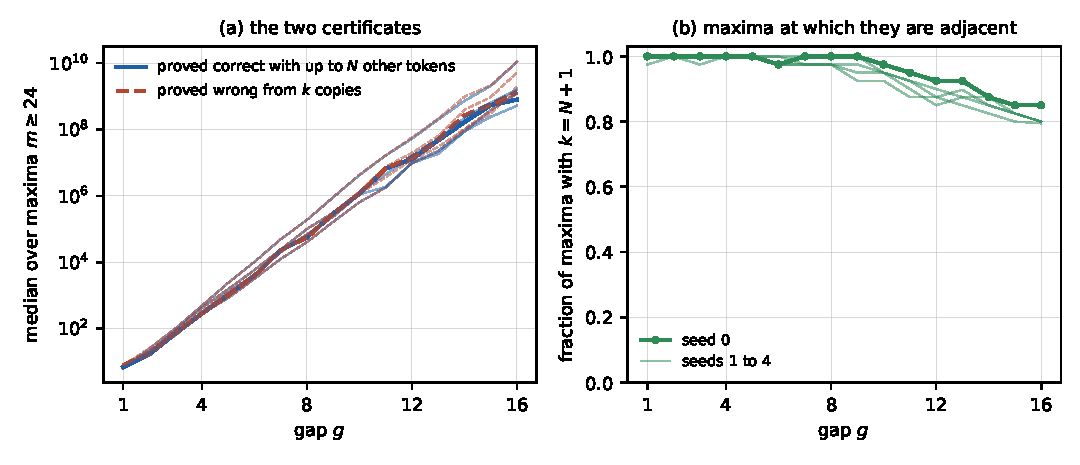
\includegraphics[width=\textwidth]{figure_gap.pdf}
\caption{(a) Median over the maxima $m\ge24$ of $N(m,g)$, the number of other
tokens at most $m-g$ that the model provably tolerates (solid), and of the
least number of copies of $m-g$ that provably defeat the maximum (dashed),
against the gap $g$; the query is the maximum. The two medians are almost
indistinguishable at this scale. (b) The fraction of maxima at which
the two numbers differ by exactly one, which are the exact thresholds of
Theorem~\ref{thm:tight}. Thick lines: seed 0; thin lines: seeds 1 to
4.}\label{fig:gap}
\end{figure}

\begin{theorem}[\lean{PF10.accuracy\_length4}, \dots, \lean{PF10.accuracy\_length100}]\label{thm:acc}
Among all $64^{n}$ inputs of length $n$, the quantised transformer answers the
maximum on a fraction of at least $0.9972$ for $n=4$, $0.9705$ for $n=10$,
$0.8841$ for $n=20$ and $0.5203$ for $n=100$. (The Lean statements give the
exact numbers of inputs.)
\end{theorem}

These bounds are conservative at long lengths. They count, for each pair of a
query and a maximum, the inputs whose other tokens lie below one threshold,
chosen so that the worst arrangement of $n-1$ such tokens is still certified.
Random long inputs almost always contain several copies of the largest tokens,
which helps the model and which this count does not use; the accuracy on random
inputs was above $0.99999$ at lengths 10 and 100. A sharper count through
Corollary~\ref{cor:counts} is a natural extension. At length 4 the bound is
close: the floating-point model answers $0.9977$ of all $64^4$ inputs
correctly, since small maxima, which it has not learned, are common at that
length.

\subsection{Seeds}

Table~\ref{tab:seeds} shows the same quantities for five training seeds.

\begin{table}[ht]
\centering
\begin{tabular}{crrrrcc}
\toprule
seed & \multicolumn{4}{c}{accuracy lower bound at length} & $N=10^6$: $(g,m_0)$ & correct exactly when\\
 & 4 & 10 & 20 & 100 & & \\
\midrule
0 & 0.9972 & 0.9705 & 0.8841 & 0.5203 & $(16,23)$ & $(20)^k\,21$: $k\le4$\\
1 & 0.9968 & 0.9638 & 0.9073 & 0.4902 & $(24,25)$ & $(20)^k\,21$: $k\le4$\\
2 & 0.9960 & 0.9682 & 0.9214 & 0.8299 & $(20,22)$ & $(23)^k\,24$: $k\le5$\\
3 & 0.9950 & 0.9660 & 0.9176 & 0.7324 & $(20,26)$ & $(28)^k\,29$: $k\le5$\\
4 & 0.9940 & 0.9680 & 0.9160 & 0.7804 & $(20,21)$ & $(28)^k\,29$: $k\le4$\\
\bottomrule
\end{tabular}
\caption{Five training seeds of the model without positional embeddings
(trained at length 10). Every entry is a kernel-checked theorem about the
quantised model of that seed. The last two columns show the row for $N=10^6$ of
the analogue of Table~\ref{tab:gap}, and one exact threshold of the analogue
of Theorem~\ref{thm:tight}: $(u)^k\,m$ means $k$ copies of $u$ followed by
$m$, and the model answers $m$ on it exactly for the values of $k$ shown. The
maximum chosen is the one that fails with the fewest copies among those covered
by the seed's first correctness statement.}\label{tab:seeds}
\end{table}

\subsection{Baseline: fixed length with positional embeddings}

To compare with Gross et al.\ in their exact setting, we also certified a model
with positional embeddings trained at length 4. Its certificate fixes the
length and searches the worst case position by position
(Appendix~\ref{app:cert}).

\begin{theorem}[\lean{K4.accuracy\_transformer}]\label{thm:k4}
The quantised transformer trained at length 4 with positional embeddings answers
the maximum on at least $16{,}777{,}215$ of the $64^4=16{,}777{,}216$ input
sequences.
\end{theorem}

The certificate consists of $2{,}079$ cases $(q,m,b)$; the single uncovered pair
$(q,m)=(0,0)$ consists of the one input $0000$, on which the floating-point
model is indeed wrong. So the bound equals the accuracy of the floating-point
model. The architecture and sizes are those of~\cite{gross2024compact}; our
model saw about 320 times as many training sequences (30{,}000 steps at batch
size 4096 against 3{,}000 at 128). Over their 151 models, of mean accuracy
$0.9992$, their brute-force proof attains the accuracy and their cubic-cost
proof strategy reports a mean bound of $0.953$, both in floating point. Our
certificate is exact and kernel-checked, and it is as tight as brute force. It
is not compact: as implemented it performs $O(V^4n^2)$ integer operations,
against $O(V^3n^2)$ floating-point operations for their cubic strategy, so at
this length it does not improve on enumeration in cost.

\subsection{Cost}

The certificates are generated in seconds. Checking them in the Lean kernel
took 43 minutes of wall-clock time for the baseline, 30 minutes for the seed-0
model without positions, and between 31 and 43 minutes for each further seed,
under four hours in all, on a desktop computer with a 24-core processor.
Each model needs between $6{,}300$ and $7{,}400$ separate kernel evaluations
(Appendix~\ref{app:lean}).

\section{What has to be trusted}\label{sec:trust}

The Lean kernel; the definitions of the real numbers and of the exponential in
Mathlib; and the definitions that the statements mention. These are the
transformer (\lean{Transformer.lean}, 100 lines); its construction from integer
weights (\lean{IntWeights} in \lean{Weights.lean},
\lean{IntWeights.toTransformer} in \lean{Link.lean}); the stored literals, that
is the weights \lean{W} (\lean{WData.lean}) and the model data \lean{M} with
the failure table \lean{nFail} (\lean{Data.lean}), the threshold table
\lean{nTight} (\lean{TightData.lean}), and the functions
\lean{unpack}, \lean{unpackInt} and \lean{allTo} that read and test them
(\lean{Check.lean}); and the short definitions \lean{query}
(\lean{Model.lean}), \lean{seqMax} (\lean{Count.lean}), \lean{IntPF.copies}
(\lean{PosFreeMain.lean}), and \lean{net}, \lean{NetAnswers} and
\lean{others} (each \lean{Main.lean}). The \lean{Main.lean} files are
generated by the certificate generator, so an auditor should read their
statements, not only check that they compile. The Python programs that train
the model and generate the certificates are not trusted for the theorems, which
speak about the integer weights written in the Lean files. They are trusted for
the separate, unproved claim that these integers are the rounded weights of the
checkpoint. The file \lean{audit/Axioms.lean} prints the axioms of 129
theorems, including every numbered result stated here and their analogues for the other
seeds; each depends on at most \lean{propext}, \lean{Classical.choice} and
\lean{Quot.sound} (28 facts about the failure and threshold tables depend on no axiom). No \lean{sorry} and no \lean{native\_decide} are used.

\section{Related work}\label{sec:related}

\paragraph{Guaranteed behaviour.}
The case for AI systems whose safety rests on machine-checkable proofs is made
in~\cite{tegmark2023provably,dalrymple2024gsai}. These proposals concern
specifications, world models and verifiers, or the replacement of learned
components by verified code, more than proofs about trained weights. Proving
properties of the learned weights themselves is the complementary problem, and
the one addressed here in miniature.

\paragraph{Robustness verification.}
Verifiers for transformers~\cite{shi2020robustness,bonaert2021deept} certify
that the output is constant on a small continuous neighbourhood of one input,
at a fixed length. Here the input space is discrete, the certified sets are
large structured families of inputs of every length, and the failure
certificates are, in effect, adversarial examples that come with a proof. The
two approaches answer different questions: local stability, and global
behaviour on a described set.

\paragraph{Proofs from mechanistic explanations.}
The programme of~\cite{gross2024compact} is the origin of this work; its proofs
are for a fixed length, in floating point, and outside a proof assistant, and
its emphasis is the trade-off between the length of a proof and the tightness of
its bound, which we do not study. It has been extended to networks trained on
group operations~\cite{wu2025groups}, and crosscoders have been proposed as the
basis of such proofs~\cite{manningcoe2026crosscoders}. Reachability analysis has
been used to bound the faithfulness of sparse replacement models under small
input perturbations~\cite{ladner2026misery}.

\paragraph{Proof assistants and trained networks.}
MLCert proved generalisation bounds for small quantised networks in
Coq~\cite{bagnall2019certifying}. Trained feed-forward classifiers have been
verified in Isabelle~\cite{brucker2023isabelle}, and the certificates produced
by a neural-network verifier can be checked by a verified
checker~\cite{desmartin2025imandra}. TorchLean formalises network semantics and
verification rules in Lean~\cite{george2026torchlean}. Closest in task and
model is a Coq development by Gross and collaborators~\cite{gross2023coqinterp},
which states the accuracy of a trained one-layer attention-only transformer on
Max-of-2 by brute-force evaluation in floating point. Closest in method is the
repository~\cite{tealsea2026}, which contains kernel-checked Lean proofs with
exact softmax that trained networks add modulo 113 on all $12{,}769$ inputs, by
enumeration, and that a trained recurrent network with five reachable states
adds binary numbers of every length. In~\cite{naughton2026verified}, a symbolic
circuit extracted from a transformer trained on bracket matching is proved in
Lean to meet its specification at every length, while the agreement of the
circuit with the trained weights is certified, by interval arithmetic outside
the proof assistant, on all inputs of one fixed length. So three kinds of
result should be kept apart: proofs about an extracted algorithm, guarantees
about the weights on a finite domain, and guarantees about the weights at every
length. Machine-checked statements about the weights of trained attention
models have so far concerned a fixed input length, and all-length statements
about the weights of trained networks have concerned recurrent networks with
finitely many reachable states; we know of none about the weights of a trained
attention model at all input lengths.

\paragraph{Length generalisation.}
There is a substantial theory of which functions transformers can represent or
learn in a way that generalises to longer
inputs~\cite{hahn2020theoretical,chiang2022overcoming,huang2025formal,yang2026bounds},
of the role of positional encodings in it~\cite{kazemnejad2023nope}, and work
that extracts programs from trained transformers~\cite{huang2026decompiling} or
synthesises and verifies transformer programs~\cite{jiang2026synthesis}. These
results concern classes of models or idealised learners, or programs rather
than weights. In their terms, Theorem~\ref{thm:gap} is a certified
length-generalisation result for one trained model. Theorem~\ref{thm:fail}
certifies failures that persist at every greater length; since they begin
below the training length, they are failures of the model and not only of its
generalisation to longer inputs. The dispersion theorem
of~\cite{velickovic2025softmax} says that with bounded scores, attention cannot
stay sharp as the input grows. That is a statement about attention weights;
whether the answer then becomes wrong depends on the values as well. For these
weights it does: on $k$ copies of $u$ followed by $m$, the sum of
Lemma~\ref{lem:sep} is $k\,e^{\sigma(m;u)}\gamma_{m,m,j}(u)+
e^{\sigma(m;m)}\gamma_{m,m,j}(m)$, and the failure certificates show that the
first term is negative for some $j$, so that it outweighs the fixed second term
once $k$ is large enough.

\section{Limitations and outlook}\label{sec:limits}

\paragraph{What the proof of concept shows.}
First, a statement about a trained transformer can be closed in a proof
assistant all the way down, at every input length, with real-valued softmax and
no trusted numerical code, in under an hour of wall-clock time per model.
Second, the statements can cover inputs of unbounded length, which no amount of
testing or enumeration can. Third, the proof is informative in both directions:
it finds inputs, at the training length, on which a model that passed random
testing is wrong, and it determines, for almost every maximum at small gaps,
the exact number of tokens at most $m-g$ that the model tolerates. A
guarantee for a deployed system would have the same shape: on every input in a
described set, the model does what it should, and outside the set there are
certified inputs on which it does not.

\paragraph{Limitations.}
\emph{Scale.} One layer, one head, no MLP, vocabulary 64. The identity of
Lemma~\ref{lem:sep} is special to a single attention layer read at one position.
For one layer without positions, verification at all lengths reduces to the
signs of finitely many linear forms in the token counts
(Corollary~\ref{cor:counts}), which is why this case is tractable. Already with
two layers, related questions are undecidable: length-generalisation bounds are
not computable for two-layer C-RASP programs~\cite{yang2026bounds}, and the
analysis of a simple class of transformers without positional encodings is
undecidable~\cite{salzer2026counting}.

\emph{The certified object.} The theorems are about the quantised model with
real arithmetic. They do not cover the floating-point checkpoint, and at long
lengths the rounding error of a floating-point softmax sum is exactly the kind of
effect that could separate the two.

\emph{Coverage.} The accuracy bounds are conservative at long lengths, and the
correctness statements start at maxima of 15 or more, which are the ones the
model has learned.

\paragraph{What scaling would need.}
Each ingredient used here has a counterpart that is open for larger models. The
\emph{specification} was trivial (the maximum of the input); for most behaviours
of interest, stating what is to be proved is the first difficulty. The
\emph{case analysis} was supplied by the identity of the tokens; in a model with
an MLP layer or several layers it would have to come from a learned
decomposition, such as a sparse dictionary, whose error is bounded for all
inputs and not only on a sample. The \emph{exact arithmetic} was affordable
because the tables are small: once the tables are linked to the weights, the
region checks grow as $V^4$ in the vocabulary ($V^2$ pairs, $V$ wrong answers,
$V$ tokens) and do not depend on $d$ or on the length. Larger models need
certified bounds that stay tight when weight matrices are composed, where Gross
et al.\ found that worst-case bounds on small unstructured residuals compound
(``structureless noise'')~\cite{gross2024compact}, and the more so through
several layers. Two next steps are concrete: a rigorous bound on the
floating-point evaluation error of the model, so that the theorems apply to the
checkpoint as it is run; and a one-layer model with an MLP, with a learned
dictionary as the skeleton of the proof.

\paragraph{Acknowledgement.}
The AI system Claude (Anthropic) assisted with development, auditing,
formalization, the computational experiments and manuscript preparation; the
author is responsible for the mathematical claims and submission.

\bibliographystyle{plain}
\bibliography{refs}

\appendix

\section{Certificate details}\label{app:cert}

\paragraph{Exponentials.}
For each query $q$ fix an integer $\bar A_q\ge A_{q,t}$ for all $t$ (the
generator takes the maximum over $t$; the kernel checks only the inequality).
The Lean function \lean{ExpBound.expBounds} computes natural numbers with
\[
 \mathrm{lo}_{q,t}\;\le\;2^{F}\exp\bigl((A_{q,t}-\bar A_q)/D\bigr)\;\le\;\mathrm{hi}_{q,t},\qquad F=256,
\]
by evaluating the Taylor polynomial of degree 39 at an argument scaled into
$[-1,0]$ in exact rational arithmetic, subtracting and adding the remainder
bound of Mathlib's \lean{Real.exp\_bound}, rounding outwards, and squaring eight
times with outward rounding (\lean{expBounds\_spec}); the same approach is used
in~\cite{tealsea2026}. The kernel evaluates this function on every entry and
compares the result with the stored literals. The $256$ fractional bits leave a
wide margin.

\paragraph{Fixed length with positional embeddings.}
Here the tables depend on the position. For a query $q$, a maximum $m$ and a
bound $b$, the checker (\lean{IntModel.check}) fixes a position for one copy of
$m$, takes at every other free position the token of $\{0,\dots,b-1\}\cup\{m\}$
that minimises the lower bound of its term, and requires the total to be
positive for every $j$ and every choice of the fixed position
(\lean{IntModel.case\_sound}). For each $j$ this is the exact worst case of the
lower bounds over all sequences with query $q$, maximum $m$ and other tokens
below $b$. The generator finds, for each $(q,m)$, the largest $b$ for which the
check passes, from prefix minima over the tokens. The tables are linked to the
weights as in the model without positions (\lean{Linked.tables\_eq}).

\paragraph{Counting.}
Let a table $\beta(q,m)\le m$ be given such that every sequence with query $q$
and maximum $m$ whose tokens all lie in $\{0,\dots,\beta(q,m)-1\}\cup\{m\}$ is
certified, for the pairs $(q,m)$ that have an entry; this set has $\beta+1$
elements. Then the number of certified sequences of length $L+1$ is
$\sum_{q,m}c_L(q,m)$, where $c_L(m,m)=(\beta+1)^L$ (the first $L$ positions are
free), $c_L(q,m)=(\beta+1)^L-\beta^L$ for $q<\beta$ (at least one of them holds
$m$), and $c_L(q,m)=0$ otherwise, in particular for a pair without an entry
(\lean{card\_covered}). The sum is evaluated by the kernel.

\paragraph{From the weights.}
The tables $A$, $B$, $U$ are stored as literals and proved equal to the
corresponding products of the integer weight matrices through intermediate
products, each a kernel-checked matrix multiplication
(\lean{Linked.tables\_eq}, \lean{LinkedPF.tables\_eq}).

\section{The Lean development}\label{app:lean}

The development has about $1{,}850$ lines of hand-written Lean on Lean~4.35.0
and Mathlib (tag \lean{v4.35.0}), and generated files with the weights, the
kernel checks and the final statements. The version described here is the
release \lean{v1.0.0} of the repository; the dependencies are pinned in
\lean{lake-manifest.json}.

\begin{center}\small
\begin{tabular}{@{}p{0.42\textwidth}p{0.54\textwidth}@{}}
\toprule
\lean{Transformer.lean} & the transformer from its weight matrices; its table form\\
\lean{Model.lean} & logits in table form; Lemma~\ref{lem:sep}\\
\lean{ExpBound.lean}, \lean{ExpCheck.lean} & integer bounds for the exponential; their check\\
\lean{Check.lean}, \lean{Sound.lean} & fixed-length checker and its soundness\\
\lean{CheckPF.lean}, \lean{PosFree.lean}, & every length: certificates\\
\lean{PosFreeMain.lean} & and their soundness\\
\lean{CheckTight.lean}, \lean{TightMain.lean} & threshold certificates and their soundness\\
\lean{Count.lean} & the number of certified sequences\\
\lean{Weights.lean}, \lean{Link.lean} & the tables as products of the weights\\
\lean{K4/}, \lean{PF10/}, \lean{PF10s1/}--\lean{PF10s4/} & generated data, kernel checks, main theorems\\
\lean{KernelBench.lean} & the kernel-speed benchmark quoted below\\
\bottomrule
\end{tabular}
\end{center}

\paragraph{Kernel evaluation.}
The checkers are plain recursive functions on integers, and each use is a
\lean{decide +kernel} of a closed proposition; \lean{native\_decide} is not used.
Two practical points decided the design. A table is stored as one natural
number and read by shifting, as in~\cite{tealsea2026}, so that an access is a
single arithmetic operation. And a single kernel evaluation had to stay small:
in a benchmark of the checker's typical step (a product of a 512-bit and a
48-bit number, a running minimum and a comparison), $10^4$ steps took 0.8\,s,
$4\times10^4$ steps 9\,s, and $6\times10^4$ steps did not finish in 90\,s (only
the first case is kept in \lean{KernelBench.lean}). The checks are therefore
split into thousands of small theorems of at most about $2\times10^4$ steps
each, $6{,}286$ for the baseline and, for each model without positions,
$6{,}268$ or $6{,}269$ together with $1{,}088$ rows of the threshold table, and
assembled by ordinary lemmas.

\paragraph{Resources.}
The times in Section~\ref{sec:results} are wall-clock times on an Intel Core
i9-13900KF (24 cores) with 32\,GB of memory. The case, region and threshold
checks do not import Mathlib and were run eight processes at a time, each under
1\,GB (the threshold checks take about three minutes per model); the
exponential-bound checks import Mathlib, each process committing 6 to 9\,GB of
virtual memory under Windows, and were run four at a time. The baseline time
covers its case and exponential checks; the linking and assembly modules add
about a minute.

\end{document}
